\documentclass{examen}
\usepackage{listings}
\begin{document}

\modulo{Lenguajes de marcas -- PARTE ORDENADOR}
\pregunta{Crea una p�gina HTML v�lida que se modifique con CSS y que contenga los siguientes
elementos
\begin{itemize}
\item{Dos encabezamientos h1 y dos encabezamientos h2. Modifica con CSS y el atributo
{\tt class} su aspecto para que aparezcan escritos con un color distinto.}
\item{Crea una lista del tipo que quieras y que tenga 3 elementos. Modifica el tipo de letra del primero y el tercero usando {\tt id}}
\item{Fabrica un enlace con el texto ``Buscador'' y que apunte a {\tt http://google.es}. Para probarlo no importa si Internet no funciona, al situar el rat�n encima el puntero cambiar� y ver�s que el navegador escribe abajo la direcci�n URL.}

\end{itemize}
}{2}

\pregunta{Elabora una p�gina HTML v�lida que contenga una tabla como la que muestra la figura siguiente}{3}

\begin{figure}[h]
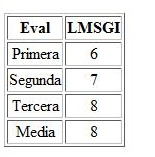
\includegraphics[scale=0.8]{examen-img/tabla.jpg}
\end{figure}

\end{document}
